% ===============================
% Document Class
% ===============================
\documentclass[12pt,a4paper,twoside]{book}

% ===============================
% Encoding & Language
% ===============================
\usepackage[T1]{fontenc}
\usepackage[utf8]{inputenc}
\usepackage[english]{babel}

% ===============================
% Page Layout
% ===============================
\usepackage{geometry}
\geometry{
    left=25mm,
    right=25mm,
    top=25mm,
    bottom=25mm
}

\usepackage{setspace}
\onehalfspacing % or \doublespacing if required

\usepackage{indentfirst}
\usepackage{pdflscape}

% ===============================
% Fonts
% ===============================
\usepackage{lmodern}        % Improved Computer Modern
\usepackage{microtype}      % Better typography

% ===============================
% Mathematics
% ===============================
\usepackage{amsmath}
\usepackage{amssymb}
\usepackage{amsfonts}
\usepackage{amsthm}
\usepackage{bm}             % Bold math symbols
\usepackage{mathtools}

% ===============================
% Graphics & Figures
% ===============================
\usepackage{graphicx}
\usepackage{float}
\usepackage{subcaption}
\usepackage{caption}
\usepackage{tikz}
\usetikzlibrary{arrows.meta,positioning,calc}

% ===============================
% Tables
% ===============================
\usepackage{booktabs}
\usepackage{multirow}
\usepackage{array}
\usepackage{longtable}
\usepackage{tabularx}

% ===============================
% Algorithms & Code
% ===============================
\usepackage{algorithm}
\usepackage{algpseudocode}

\usepackage{listings}
\usepackage{xcolor}

\lstset{
    basicstyle=\ttfamily\small,
    keywordstyle=\color{blue},
    commentstyle=\color{gray},
    stringstyle=\color{red},
    numbers=left,
    numberstyle=\tiny,
    frame=single,
    breaklines=true
}

% ===============================
% Units & Symbols
% ===============================
\usepackage{siunitx}
\sisetup{
    per-mode=symbol,
    detect-all
}

% ===============================
% Hyperlinks
% ===============================
\usepackage{hyperref}
\hypersetup{
    colorlinks=true,
    linkcolor=blue,
    citecolor=blue,
    urlcolor=blue
}


% ===============================
% Chapter/Section appearance
% ===============================
\usepackage{titlesec}

% Chapters: small "Chapter X", big title, better spacing
\titleformat{\chapter}[display]
  {\normalfont\bfseries}
  {\Large\chaptername\ \thechapter}
  {5ex}
  {\huge}

\titlelabel{\thetitle.\quad} % aggiunge un punto dopo il numero di sezione

% ===============================
% Headings & TOC
% ===============================
\usepackage{chngcntr} % for \counterwithin
\usepackage{tocloft}
\usepackage{fancyhdr}
\pagestyle{fancy}
\fancyhf{}

% -----------------------
% Marks (chapter/section)
% -----------------------
% Ogni volta che inizia un capitolo, imposta i marcatori dell'intestazione:
% \leftmark  = "numero. titolo del capitolo" (es. "2. Contesto storico")
% \rightmark = vuoto (azzera la sezione precedente)
\renewcommand{\chaptermark}[1]{\markboth{\thechapter.\ #1}{}}

% Ogni volta che inizia una sezione, aggiorna solo il marcatore destro:
% \rightmark = "numero. titolo della sezione" (es. "2.1. Le equazioni di Maxwell")
% \leftmark resta invariato (capitolo corrente)
\renewcommand{\sectionmark}[1]{\markright{\thesection.\ #1}}

% -----------------------
% Header
% -----------------------
% Left: capitolo corrente (il numero di pagina NON sta più qui)
\fancyhead[L]{\small\nouppercase{\leftmark}}

% -----------------------
% Footer: solo numero di pagina al centro
% -----------------------
\fancyfoot[C]{\thepage}

% -----------------------
% Lines
% -----------------------
\renewcommand{\headrulewidth}{0.4pt}
\renewcommand{\footrulewidth}{0pt}

% -----------------------
% First page of chapters
% -----------------------
\fancypagestyle{plain}{
\fancyhf{}
\fancyfoot[C]{\thepage}
\renewcommand{\headrulewidth}{0pt}
\renewcommand{\footrulewidth}{0pt}
}

% -----------------------
% Unnumbered chapters
% -----------------------
\fancypagestyle{chapterstar}{
\fancyhf{}
\fancyfoot[C]{\thepage}
\renewcommand{\headrulewidth}{0pt}
\renewcommand{\footrulewidth}{0pt}
}

% -----------------------
% Prima pagina dei capitoli
% -----------------------
\fancypagestyle{chapterplain}{
\fancyhf{}
\fancyfoot[C]{\thepage}
\renewcommand{\headrulewidth}{0pt}
\renewcommand{\footrulewidth}{0pt}
}

% -----------------------
% Pagine interne dei capitoli
% -----------------------
\fancypagestyle{chapternum}{
  \fancyhf{}

  % Header: sezione corrente a sinistra
  \fancyhead[L]{\small\rightmark}

  % Footer: numero di pagina al centro
  \fancyfoot[C]{\thepage}

  \renewcommand{\headrulewidth}{0.4pt}
  \renewcommand{\footrulewidth}{0pt}
}


% ===============================
% Appendices
% ===============================
\usepackage{appendix}

% ===============================
% Nomenclature / Acronyms
% ===============================
\usepackage{nomencl}
\makenomenclature

% \usepackage[acronym]{glossaries}
% \makeglossaries

% ===============================
% PDF Inclusion
% ===============================
\usepackage{pdfpages}

% ===============================
% Line Breaking & Widow Control
% ===============================
\usepackage[all]{nowidow}

% ===============================
% Custom Commands (optional)
% ===============================
% \newcommand{\R}{\mathbb{R}}
% \newcommand{\vect}[1]{\boldsymbol{#1}}

% \newcommand{\AuthorName}{\textit{X.Y.Surname}}
% \newcommand{\ThesisTitle}{Title of Thesis}
% \newcommand{\CourseUniversity}{BSc/MSc, Course, Department, University of Bologna}

\setlength{\headheight}{14pt}

% ===============================
% End of Preamble
% ===============================


\begin{document}

    %Only for title page 
    \setlength{\parindent}{15pt}
    \setlength{\parskip}{15mm}
    
    \begin{titlepage}
        \begin{center}
            % include il logo che si trova nella cartella immagini
            % 
\includegraphics[width = 6.5cm, height = 6.5cm]{immagini/Unibo_logo.png}
            
            {\Large{\bf{Laurea Magistrale in Didattica, Storia ed Epistemologia della Fisica}}}
        
            {\bfseries\fontsize{26pt}{20pt}\selectfont
                \setlength{\lineskip}{2pt}%
                \setlength{\lineskiplimit}{0pt}%
                Onde elettromagnetiche: l'analogia con l'ottica\par}
            
        \end{center}

\vfill

% Qui sotto c'è la parte di testo che appare in basso a sinistra e a destra della pagina del frontespizio,
% con i nomi del relatore, correlatore e laureando. Puoi modificare i nomi come preferisci.
\begin{minipage}[t]{0.5\textwidth}
    {\Large{\bf Relatore: \\ Prof. Eugenio Bertozzi}}
    \vspace{6mm}

    {\Large{\bf Correlatore: \\ Non Pervenuto}}
    
\end{minipage}
\hfill
\begin{minipage}[t]{0.40\textwidth}\raggedleft
    {\Large{\bf Laureando: \\ Leonardo Amadori}}
\end{minipage}

\rule[0.5mm]{15.3845cm}{0.4mm}
\vspace{-\baselineskip}
\begin{center}
    % {\large\bfseries Graduation Session Month 20XX\\}
    {\large\bfseries Anno Accademico 2025/2026}
\end{center}

    \end{titlepage}
    \clearpage{\pagestyle{empty}\cleardoublepage}

    \pagenumbering{roman} %page numbering is roman letters for this section
    \setlength{\parindent}{15pt}
    \setlength{\parskip}{0pt}
    
    % ==============================
    % Abstract
    % ==============================
	% \chapter*{Abstract}
    % \addcontentsline{toc}{chapter}{Abstract}
    % \thispagestyle{chapterstar}
	% \label{abstract_Eng}
	% % \input{Abstract_Eng.tex}
	% \clearpage{\pagestyle{empty}\cleardoublepage} % sezione inattiva perché la tesi è in italiano, ma se vuoi puoi attivarla togliendo il commento

    % ==============================
    % Riassunto (abstract in Italiano)
    % ==============================
	\chapter*{Riassunto}
    \addcontentsline{toc}{chapter}{Riassunto}
    \thispagestyle{chapterstar}
	\label{abstract_It}
	% \input{Abstract_It.tex}
	\clearpage{\pagestyle{empty}\cleardoublepage}
	
	% ==============================
    % indice
    % ==============================
    \tableofcontents
    \thispagestyle{chapterstar}
    \clearpage
    \pagestyle{fancy}
    \cleardoublepage

    % ==============================
    % lista delle figure
    % ==============================
    \addcontentsline{toc}{chapter}{List of Figures}
	\listoffigures
    \thispagestyle{chapterstar}
	\clearpage{\pagestyle{empty}\cleardoublepage}

    % ==============================
    % Lista delle tabelle
    % ==============================
    % \listoftables
    % \thispagestyle{chapterstar}
    % \addcontentsline{toc}{chapter}{List of Tables}
    % \clearpage{\pagestyle{empty}\cleardoublepage}

    % ==============================
    % Nomenclatura
    % ==============================
    % \chapter*{Nomenclature}
    % \addcontentsline{toc}{chapter}{Nomenclature}
    % \thispagestyle{chapterstar}
	% \label{Nomencla}
	% % \input{Nomenclature}
    % \clearpage{\pagestyle{empty}\cleardoublepage}

    \mainmatter % Now Use Arabic numerals for page numbers 
    \pagestyle{chapternum} % uso lo stile di intestazione per le pagine interne dei capitoli, con il numero di pagina al centro del piè di pagina
    
    \pagenumbering{arabic}
    
    % ==============================
    % Introduzione
    % ==============================
	% \chapter{Introduction}
    \thispagestyle{chapterplain}
	\label{chap:introduzione}
    \chapter*{Introduzione}
\addcontentsline{toc}{chapter}{Introduzione}

Questo capitolo introduce il lavoro di Tesi.
Chi era Augusto righi? E perché è importante studiare la sua vita e le sue opere?
In questa tesi si vuole analizzare gli esperimenti condotti dal Fisico italiano, 
uno dei pionieri nello studio delle onde elettromagnetiche.
Righi scrisse il seguente testo: \cite{righi1897ottica}
% \section{Obbiettivi del lavoro}

Testo della seconda sezione.

% \begin{figure}[htbp]
%   \centering
%   \includegraphics[width=0.7\textwidth]{nome-immagine.png}
%   \caption{Didascalia della figura.}
% \end{figure} % INTRODUZIONE DA ALTRO FILE
	\clearpage{\pagestyle{empty}\cleardoublepage}
	
    % ==============================
    % Capitolo 1: Contesto Storico
    % ==============================
    % \chapter{Contesto Storico}
    \thispagestyle{chapterplain}
    \label{chap:contesto_storico}
	\chapter{Contesto Storico}
% \addcontentsline{toc}{chapter}{Contesto Storico}

il contesto storico degli esperimenti sulle
onde elettromagnetiche condotti alla fine dell'Ottocento~\cite{righi1897ottica}.

Come evidenziato da Bertozzi \cite{bertozzi2020augusto}, Righi fu un fisico italiano che visse in un periodo 
di grande fermento scientifico e tecnologicoDragoni~\cite{dragonirighi2023}.
% \section{Contesto storico}

Qui scrivi il testo della prima sezione. Puoi usare tutti i comandi
che useresti in \texttt{main.tex}: formule, elenchi, citazioni e così via.
 % CONTEXTO STORICO DA ALTRO FILE
	\clearpage{\pagestyle{empty}\cleardoublepage}
	
    % ==============================
    % nuovo capitolo
    % ==============================
    \chapter{Teoria delle onde elettromagnetiche}
    % \thispagestyle{chapterplain}
    \label{chap:teoria_onde_em}
	% \chapter*{Teoria delle onde elettromagnetiche}
% \addcontentsline{toc}{chapter}{Teoria delle onde elettromagnetiche}

Le equazioni di maxwell nel vuoto sono le seguenti:

\begin{subequations}\label{eq:maxwell}
\begin{align}
\vec{\nabla} \cdot \vec{E} &= 0 \label{eq:maxwell-gauss-e}\\
\vec{\nabla} \cdot \vec{B} &= 0 \label{eq:maxwell-gauss-b}\\
\vec{\nabla} \times \vec{E} &= -\frac{\partial \vec{B}}{\partial t} \label{eq:maxwell-faraday}\\
\vec{\nabla} \times \vec{B} &= \mu_0 \varepsilon_0 \frac{\partial \vec{E}}{\partial t} \label{eq:maxwell-ampere}
\end{align}
\end{subequations}

Per dimostrare che le equazioni di Maxwell implicano l'esistenza di onde elettromagnetiche, bisogna manipolarle fino ad ottenere 
un'equazione differenziale nella forma dell'equazione di d'Alembert.\\
Iniziamo prendendo il rotore di \eqref{eq:maxwell-faraday}:

\begin{equation}\label{eq:maxwellxrotor}
\vec{\nabla} \times (\vec{\nabla} \times \vec{E}) = -\frac{\partial}{\partial t} (\vec{\nabla} \times \vec{B})
\end{equation}

per risolvere il membro di sinistra, possiamo usare l'identità vettoriale:
\begin{equation}    
    \vec{A} \times (\vec{B} \times \vec{C}) = \vec{B} (\vec{A} \cdot \vec{C}) - \vec{C} (\vec{A} \cdot \vec{B})
\end{equation}

che applicata al nostro caso diventa:
\begin{equation}
    \vec{\nabla} \times (\vec{\nabla} \times \vec{E}) = \vec{\nabla} (\vec{\nabla} \cdot \vec{E}) - \vec{\nabla}^2 \vec{E}
\end{equation}
ora, dalla \eqref{eq:maxwell-gauss-e} sappiamo che $\vec{\nabla} \cdot \vec{E} = 0$, quindi il primo termine del membro di 
sinistra si annulla e rimane:  
\begin{equation}
    \vec{\nabla} \times (\vec{\nabla} \times \vec{E}) = - \vec{\nabla}^2 \vec{E}
\end{equation}
quindi il membro di sinistra della \eqref{eq:maxwellxrotor} diventa:
\begin{equation}
    - \vec{\nabla}^2 \vec{E} = -\frac{\partial}{\partial t} (\vec{\nabla} \times \vec{B})   
\end{equation}
ora, sostituendo il membro di destra della \eqref{eq:maxwellxrotor} con la \eqref{eq:maxwell-ampere}, otteniamo:
\begin{equation}
    - \vec{\nabla}^2 \vec{E} = -\mu_0 \varepsilon_0 \frac{\partial^2 \vec{E}}{\partial t^2}
\end{equation}
che può essere riscritta come:
\begin{equation}
    \vec{\nabla}^2 \vec{E} - \mu_0 \varepsilon_0 \frac{\partial^2 \vec{E}}{\partial t^2} = 0
\end{equation}
questa è l'equazione di d'Alembert per il campo elettrico.\\ 
Un ragionamento analogo può essere condotto per il campo magnetico, ottenendo un'equazione simile.
	% \clearpage{\pagestyle{empty}\cleardoublepage}

    % ==============================
    % nuovo capitolo
    % ==============================
    \chapter{Esperimenti}
    \thispagestyle{chapterplain}
    \label{chap:Esperimenti}
	% \input{Chapter3}
	\clearpage{\pagestyle{empty}\cleardoublepage}
	\section{Esperienza \S~38}

L'esperienza del \S~38, descritta nel capitolo V del volume di Righi~\cite{righi1897ottica} (pagina 148 del libro), 
ha per oggetto la riflessione delle onde elettromagnetiche. Prima di descriverla è però opportuno richiamare il 
concetto di riflessione (fig \ref{fig:riflessione_theta}) e la legge che la governa.\\
Tale legge afferma che l'angolo di incidenza di un raggio luminoso è uguale all'angolo di riflessione:
\begin{equation}
    \theta_i = \theta_r .
    \label{eq:legge-riflessione}
\end{equation}

La sua formulazione più antica è tradizionalmente attribuita a Euclide (circa 300~a.C.), nel trattato di Ottica.\\ 
La legge di riflessione come la conosciamo oggi è:

\begin{figure}[htbp]
    \centering
    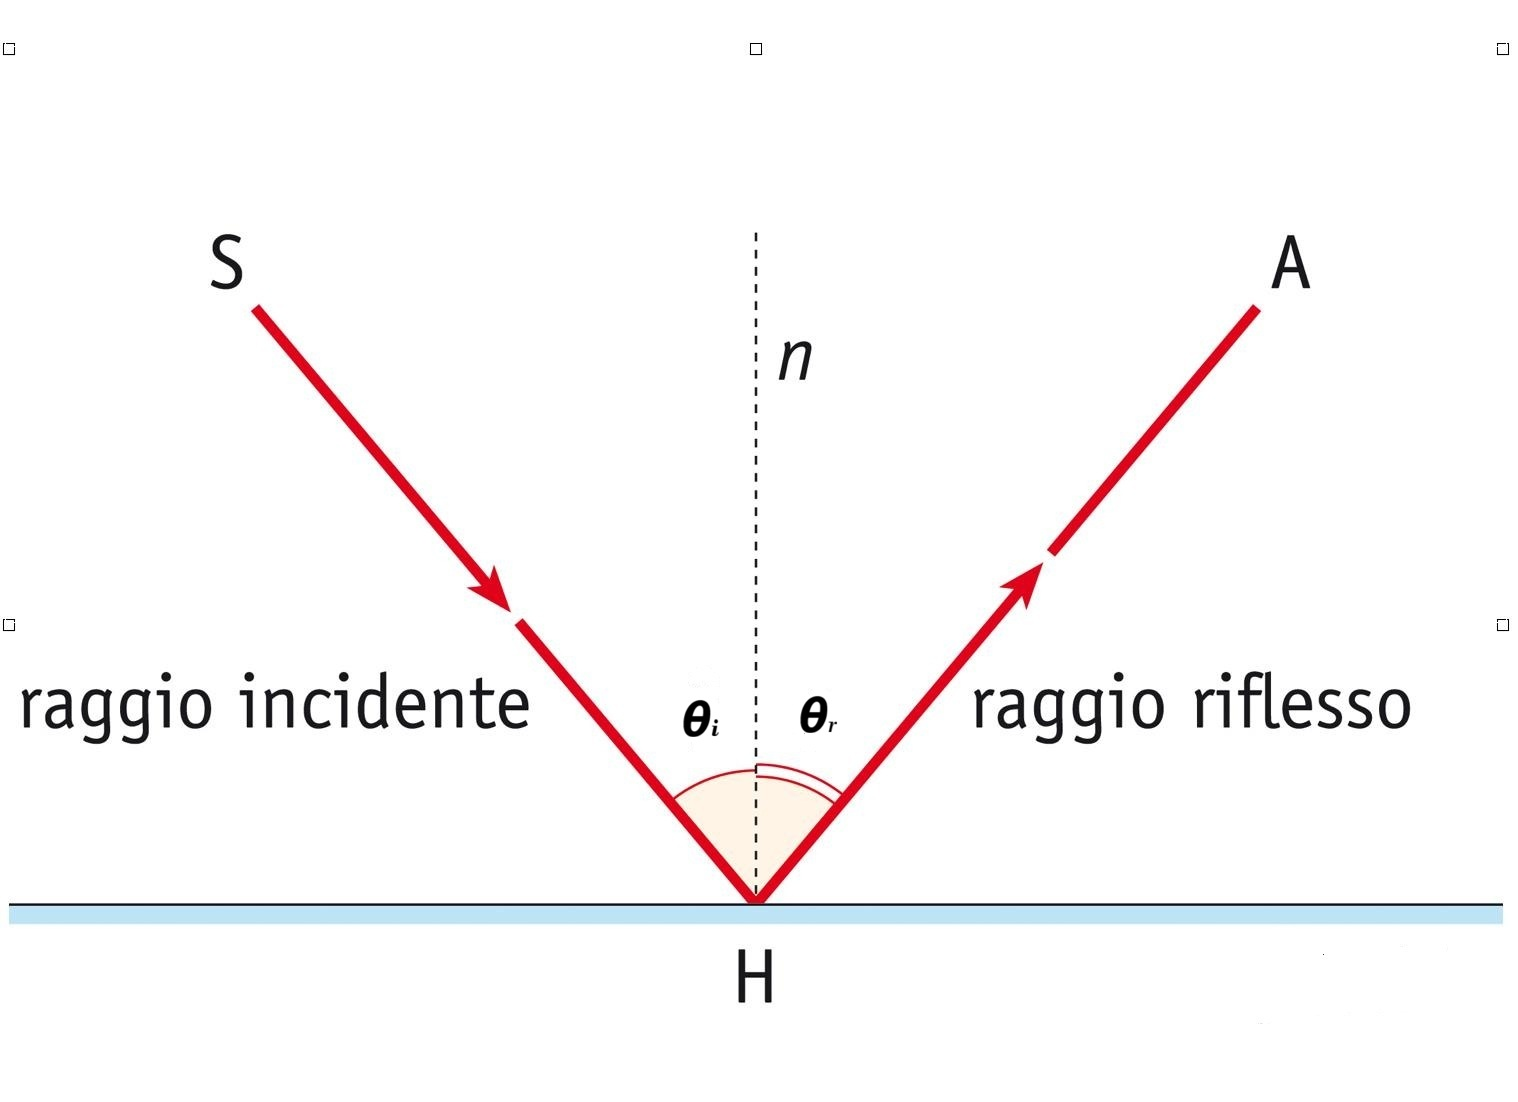
\includegraphics[width = 0.8\textwidth]{immagini/riflessione_theta.jpg}
    \caption{Schema della legge di riflessione}
    \label{fig:riflessione_theta}
\end{figure}

\subsection{Set up sperimentale}

La descrizione dell'esperimento inizia con "specchi sferici concavi di metallo" di 44 cm di diametro e 18.6 cm di distanza focale ($f$),
inizialmente "\textit{adoperati nelle lezioni per la riflessione del suono e del calore}". \\
Ragionando in 2-D (fig \ref{fig:specchio_concavo}) e usando la trigonometria risulta che:
\begin{itemize}
    \item il raggio di curvatura ($R$) dello specchio è $R = 2f = 37.2$ cm, 
    \item il semiangolo di apertura dello specchio è $\alpha = \arcsin{\frac{D/2}{R}} \approx 36^\circ$.
\end{itemize}

\begin{figure}[htbp]
    \centering
    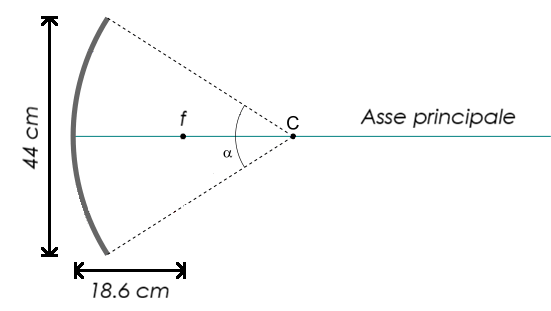
\includegraphics[width = 0.8\textwidth]{immagini/schema_specchio_concavo.png}
    \caption{Schema dello specchio concavo}
    \label{fig:specchio_concavo}
\end{figure}

Tornando all'esperienza di Righi, l'apparato sperimentale da lui impiegato per la verifica della legge di riflessione è il seguente:

\begin{itemize}
    \item \textbf{Emettitore/Oscillatore ($O$)}: un oscillatore a quattro sfere con le due centrali immerse in olio di vaselina (ideato dal fisico bolognese stesso), posizionato lungo la linea focale di uno specchio cilindrico parabolico di rame ($M_1$). Tale riflettore concentra l'energia emessa proiettando uno stretto fascio di radiazioni parallele e linearmente polarizzate.
    \item \textbf{Superficie riflettente ($S$)}: un'ampia lastra piana (metallica o di materiale dielettrico come vetro o paraffina) disposta verticalmente al centro di una piattaforma goniometrica graduata ($P$). La lastra può essere ruotata per impostare con precisione l'angolo di incidenza $\theta_i$ rispetto alla normale $N$ alla superficie.
    \item \textbf{Rilevatore/Risonatore ($R$)}: un risonatore a striscia d'argento interrotta, posto nel fuoco di un secondo specchio cilindrico parabolico ($M_2$). Questo secondo specchio è montato su un braccio metallico orientabile che ruota attorno all'asse centrale del goniometro $P$, consentendo di misurare l'intensità del segnale riflesso a qualsiasi angolo $\theta_r$.
\end{itemize}

\begin{figure}[htbp]
    \centering
    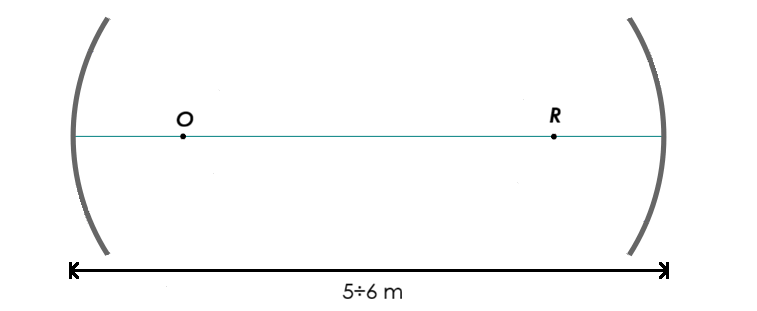
\includegraphics[width = 0.8\textwidth]{immagini/schema_esp_base.png}
    \caption{Schema dell'apparato sperimentale: O è l'oscillatore, R è il risonatore.}
    \label{fig:setup-base}
\end{figure}

% \begin{figure}[htbp]
%     \centering
%     \includegraphics[width = 0.85\textwidth]{immagini/setup_esperimento_38.png}
%     \caption{Schema dell'apparato sperimentale adoperato da Righi per la verifica delle leggi della riflessione ($\theta_i = \theta_r$).}
%     \label{fig:setup-riflessione}
% \end{figure}

Durante l'esecuzione dell'esperienza, inviando il fascio incidente con un angolo $\theta_i$ prefissato e facendolo incidere sulla lastra $S$, Righi ruota il braccio del risonatore $R$ registrando la brillantezza delle scintille. La massima luminosità della scarica si osserva con rigorosa precisione \textbf{esclusivamente quando l'angolo di riflessione coincide con l'angolo di incidenza} ($\theta_r = \theta_i$). Inoltre, spostando il risonatore al di sopra o al di sotto del piano d'incidenza orizzontale, le scintille cessano immediatamente, confermando sperimentalmente che il raggio riflesso giace nello stesso piano individuato dal raggio incidente e dalla normale alla superficie \cite{righi1897ottica}.

\paragraph{Analogia con la conduzione in tubo metallico.}
A completamento del \S~38, Righi descrive un'ulteriore ed elegante esperienza in cui colloca l'oscillatore all'estremità di un lungo tubo metallico cavo (simile a un comune tubo da stufa) e il risonatore all'estremità opposta. Le pareti metalliche interne fungono da specchio continuo, guidando l'onda elettromagnetica per successive riflessioni speculari interne senza dispersione spaziale (primo esempio di \emph{guida d'onda}). L'interruzione della radiazione mediante un disco conduttore interno ne conferma la natura di riflessione confinata, in perfetta analogia con la propagazione del suono nei tubi acustici o della luce in condotti a specchio \cite{righi1897ottica}.

\subsection{Considerazioni fisiche e implicazioni teoriche}

Dopo aver verificato le leggi puramente geometriche dell'ottica, Righi compie un fondamentale passaggio concettuale: dallo studio \emph{geometrico} della traiettoria dei raggi passa allo studio \emph{fisico} della natura vettoriale delle oscillazioni riflesse, analizzandone l'intensità, lo stato di fase e l'orientazione nello spazio \cite{righi1897ottica}.

\subsection{Naturale polarizzazione e prova della teoria di Maxwell}
Mentre la luce naturale visibile è emessa con piani di vibrazione casuali e disordinati, le onde elettromagnetiche generate dagli oscillatori a scarica nascono \textbf{intrinsecamente e totalmente polarizzate} rettilinealmente, con la direzione del campo elettrico definita dall'asse dell'oscillatore \cite{righi1897ottica}.

Questa proprietà permette a Righi di impostare un test cruciale per confrontare la teoria ottica ondulatoria classica di Fresnel con la teoria elettromagnetica di Maxwell \cite{righi1897ottica}:
\begin{itemize}
    \item Nella teoria elastica di Fresnel, la vibrazione dell'etere avvenga in direzione \emph{perpendicolare} al piano di polarizzazione.
    \item Nella teoria di Maxwell, il campo elettromagnetico è costituito da due vettori ortogonali: la forza elettrica ($\mathbf{E}$) e la forza magnetica ($\mathbf{H}$).
\end{itemize}
Righi dimostra sperimentalmente che la \textbf{forza elettrica corrisponde esattamente alla vibrazione dell'etere della teoria di Fresnel} (risultando perpendicolare al piano di polarizzazione), mentre la \textbf{forza magnetica giace nel piano di polarizzazione} \cite{righi1897ottica}. Questo risultato fornisce una conferma sperimentale diretta dell'identità tra vibrazioni luminose e oscillazioni elettromagnetiche \cite{righi1897ottica, righi1897ottica}.

\subsection{Fondamento per i fenomeni complessi della riflessione}
La verifica condotta nel \S~38 costituisce il presupposto metodologico per le indagini svolte nei paragrafi successivi del Capitolo V \cite{righi1897ottica}:
\begin{enumerate}
    \item \textbf{Riflessione sui dielettrici (\S~39--40)}: studio della variazione d'intensità dell'onda riflessa al variare dell'angolo d'incidenza su isolanti (vetro, paraffina, zolfo) e verifica dell'estinzione dell'onda all'\emph{angolo di Brewster}, confermando le formule di Fresnel.
    \item \textbf{Riflessione metallica ed ellittica (\S~41--43)}: analisi dello sfasamento introdotto dalla riflessione sui conduttori metallici (rame), che trasforma un'onda a polarizzazione rettilinea in un'onda a \emph{polarizzazione ellittica o circolare}.
\end{enumerate}

Attraverso queste esperienze, Righi dimostra che la riflessione delle onde radio segue in tutto e per tutto le medesime leggi e relazioni quantitative stabilite da Fresnel e Malus per la luce visibile, consolidando la sintesi elettromagnetica di Maxwell \cite{righi1897ottica}.


	% ==============================
    % nuovo capitolo
    % ==============================	
    \chapter{Experimental Setup}
    \thispagestyle{chapterplain}
    \label{chap:experimental-setup}
	% \input{Chapter4}
	\clearpage{\pagestyle{empty}\cleardoublepage}
	
	% ==============================
    % nuovo capitolo
    % ==============================
    \chapter{Results and Discussion}
    \thispagestyle{chapterplain}
    \label{chap:results}
	% \input{Chapter5}
	\clearpage{\pagestyle{empty}\cleardoublepage}
	
	
    % ==============================
    % conclusioni
    % ==============================
	\chapter{Conclusions}
    \thispagestyle{chapterplain}
	\label{chap:conclusion}
	% \input{Conclusion}
	\clearpage{\pagestyle{empty}\cleardoublepage}

    	
    \pagestyle{plain}
    \cleardoublepage
    \setcounter{page}{1}
    \renewcommand{\thepage}{B\arabic{page}}

    % ==============================
    % Ringraziamenti
    % ==============================
    \pagestyle{chapterstar}
    \chapter*{Ringraziamenti}
    \addcontentsline{toc}{chapter}{Ringraziamenti}
    \thispagestyle{chapterstar}
	\label{ringraziamenti}
	% \input{Acknowledgment}
	\clearpage{\pagestyle{empty}\cleardoublepage}

    % ==============================
    % Bibliografia
    % ==============================
    \bibliographystyle{ieeetr}
    \addcontentsline{toc}{chapter}{bibliografia}
    \bibliography{bibliografia}

\end{document}